\documentclass[conference]{IEEEtran}
% Short paper (progress report). Build: pdflatex short_paper; bibtex short_paper; pdflatex short_paper (x2)
% All numbers, tables and plots come from analysis/make_figures.py run on the experiment database.
% The Word version (short_paper.docx) is built from the same text by analysis/make_docx.js.
\usepackage[T1]{fontenc}
\usepackage{cite}
\usepackage{amsmath,amssymb}
\usepackage{graphicx}
\usepackage{booktabs}
\usepackage{xcolor}
\usepackage{tikz}
\usetikzlibrary{arrows.meta,positioning,fit,calc,backgrounds}
\usepackage{url}
\usepackage[hidelinks]{hyperref}
\usepackage{microtype}

\definecolor{cUrdu}{HTML}{009E73}
\definecolor{cRoman}{HTML}{D55E00}
\definecolor{cMixed}{HTML}{CC79A7}
\definecolor{cEng}{HTML}{0072B2}
\definecolor{cInk}{HTML}{333333}
\definecolor{cBox}{HTML}{F4F6F8}

\newcommand{\rom}[1]{\textit{#1}}  % Roman-Urdu text

\begin{document}

\title{Is the AI Judge Fair to Roman Urdu?\\ Measuring Script Bias in LLM Judges}

\author{\IEEEauthorblockN{Saif ur Rehman (24280071),\; Hussnain Ali Murtaza (25280069),\; Syed Sheraz Anjum (25240017),\\
Junaid Tariq (25280044),\; Mukhammad Khasnen (25280090)}
\IEEEauthorblockA{2601 SSE Responsible AI Engineering, Group 10 \\
Lahore University of Management Sciences (LUMS), Lahore, Pakistan}}

\maketitle

\begin{abstract}
LLMs are often used as judges to mark answers. Many Urdu speakers write Urdu in English letters (Roman Urdu) and mix in
English words, but we do not know if LLM judges mark these answers as fairly as answers in Urdu script. We took 300
reading questions from the Belebele dataset and wrote each answer in Urdu script, Roman Urdu, Urdu--English mixed text
and English. The meaning stayed the same in all four. Nine judges from three companies, in three model sizes, marked and
compared these answers. Every judge that passed our first check gave the same correct answer 0.55 to 1.26 marks less
(out of 10) in Roman Urdu than in Urdu script, and 0.59 to 1.30 marks less in mixed text. English answers got more
marks. We saw the same gap when we repeated the test, and also on questions the judge had understood in both scripts.
Bigger models did not have a smaller gap. Of the fixes we tried, changing the answer into Urdu script before judging
helped the most.
\end{abstract}

\begin{IEEEkeywords}
LLM-as-a-judge, fairness, script bias, Roman Urdu, code-mixing
\end{IEEEkeywords}

% =====================================================================
\section{Introduction}
LLM judges are now used a lot to check the work of other AI systems. They mark answers, rank chatbot replies and help
train other models \cite{zheng2023judging}. A fair judge should mark an answer only on what it says. Past studies show
this does not always happen. Judges like their own answers more \cite{panickssery2024llm}, like text that looks familiar
to them \cite{wataoka2024self} and change their decision after small edits to the input \cite{ye2025justice}.

Urdu is an interesting case because people write it in two scripts. Books and newspapers use Urdu script
(\raisebox{-0.3ex}{
\includegraphics[height=1.9ex]{figures/urdu_example.pdf}}, ``five villages''), but on phones and
social media many people type Roman Urdu (\rom{paanch dehaat}). They often mix in English words too
(\rom{paanch villages}). Roman Urdu also has no fixed spelling \cite{khan2022clustering}. If a judge gives fewer marks
to a correct answer just because it is in Roman Urdu, then any marking tool built on that judge is unfair to a very large
number of users.

So our main question is this: if the meaning of an answer stays the same, does its script change how an LLM judge marks
it, compares it and understands it? We look at three parts. Is there a gap (RQ1)? Is the gap only because the judge
understands Roman Urdu less well (RQ2)? Does the gap get smaller with bigger models or with simple fixes (RQ3)?

% =====================================================================
\section{Related Work}
Our method follows CALM \cite{ye2025justice}. CALM changes one thing in the input at a time and checks if the judge's
decision changes. It covers twelve types of bias, but script is not one of them. Studies on familiar text and on judges
preferring their own answers \cite{panickssery2024llm,wataoka2024self} may explain script bias, but for now this is only
an idea we will test.

Judges are also less reliable outside English. Fu and Liu found that judges agree less with each other in 25 languages,
and least in languages with little training data \cite{fu2025reliable}. Zhou et al.\ found that the same content gets
different marks in different languages \cite{zhou2026lower}. MM-Eval \cite{son2026mmeval} and the CIA suite
\cite{doddapaneni2025cross} test judges in many languages, and Hada et al.\ suggest checking them against native speakers
\cite{hada2024large}. All of these studies compare languages. We compare two scripts of one language.

Results on Roman script are mixed. For Indian languages, the script changed how well models sorted patient messages
\cite{khullar2026script}, but U-MIRAGE found that Roman Urdu did better than Urdu script on medical questions
\cite{faheem2026umirage}. RomanSetu \cite{husain2024romansetu}, RomanLens \cite{saji2025romanlens} and a study of Roman
Urdu and safety \cite{jamil2026code} look at what models can do or at safety. They do not look at marking. Work on dialect \cite{faisal2025dialectal,hofmann2024ai}, mixed text
\cite{yang2025codemixbench,mohamed2025lost,gupta2026code} and Urdu grammar \cite{adeeba2026urblimp} is also related. As far as we know, no study has checked whether an LLM judge marks the same Urdu answer
differently when only the script changes.

% Fig. 1: study design (TikZ). Included from short_paper.tex.
\begin{figure*}[t]
\centering
\resizebox{\textwidth}{!}{%
\begin{tikzpicture}[
  font=\footnotesize, >={Stealth[length=2.2mm]},
  stage/.style={draw=cInk!45, rounded corners=3pt, fill=cBox, inner sep=4pt, align=left, anchor=north west},
  head/.style={font=\footnotesize\bfseries, anchor=south west, inner sep=1pt},
  ver/.style={rounded corners=2pt, inner sep=2.5pt, text width=2.95cm, align=left, font=\scriptsize, text=white},
  arr/.style={->, thick, cInk!70}]
% Stage 1
\node[stage, text width=2.7cm, minimum height=3.35cm] (s1) at (0,0) {%
  \textbf{Belebele item}\\[2pt]
  Passage ($\approx$100 words)\\ Question\\ 4 answer options\\[3pt]
  300 items (seed 13)\\ $\rightarrow$ correct option\\ $\rightarrow$ one wrong option};
\node[head] at (s1.north west) {\textcolor{cInk}{\textsf{1} Data}};
% Stage 2: four versions
\node[stage, text width=3.25cm, minimum height=3.35cm] (s2) at (3.35,0) {};
\node[anchor=north west, inner sep=0pt] at ($(s2.north west)+(0.14,-0.14)$) {\textbf{Same answer, four scripts}};
\node[head] at (s2.north west) {\textcolor{cInk}{\textsf{2} Versions}};
\node[ver, fill=cUrdu, anchor=north] (v1) at ($(s2.north)+(0,-0.55)$) {Urdu script\hfill\raisebox{-0.25ex}{\colorbox{white}{
\includegraphics[height=1.55ex]{figures/urdu_example.pdf}}}};
\node[ver, fill=cRoman, below=2.5pt of v1] (v2) {Roman Urdu\hfill \rom{paanch dehaat}};
\node[ver, fill=cMixed, below=2.5pt of v2] (v3) {Code-mixed\hfill \rom{paanch villages}};
\node[ver, fill=cEng, below=2.5pt of v3] (v4) {English\hfill Five villages};
\node[font=\scriptsize, align=left, text width=3.1cm, below=3pt of v4, text=cInk] {Belebele's own: \rom{Paanch gaon}\\ \textcolor{cRoman}{reworded $\Rightarrow$ not used}};
% Stage 3: judges, a company x size grid
\node[stage, text width=3.6cm, minimum height=3.35cm] (s3) at (7.25,0) {};
\node[anchor=north west, inner sep=0pt] at ($(s3.north west)+(0.14,-0.14)$) {\textbf{9 judges, 3 companies}};
\node[head] at (s3.north west) {\textcolor{cInk}{\textsf{3} Judges}};
\foreach \x/\fam in {8.3/Alibaba, 9.4/Meta, 10.5/Google}
  \node[font=\scriptsize\bfseries, text=cInk] at (\x,-0.78) {\fam};
\foreach \y/\tier in {-1.2/S, -1.72/M, -2.24/L}
  \node[font=\scriptsize\bfseries, text=cInk] at (7.6,\y) {\tier};
\foreach \x/\y/\m in {8.3/-1.2/Qwen3.5 9B, 9.4/-1.2/Llama 3.1 8B, 10.5/-1.2/Gemma 3 12B,
                      8.3/-1.72/Qwen3 32B, 9.4/-1.72/Llama 3.3 70B, 10.5/-1.72/Gemma 3 27B,
                      8.3/-2.24/Qwen3 235B, 9.4/-2.24/Llama 4 Maverick, 10.5/-2.24/Gemini 2.5 Flash}
  \node[draw=cInk!30, fill=white, rounded corners=1.5pt, font=\tiny, align=center, text width=0.92cm,
        minimum height=0.44cm, inner sep=1pt] at (\x,\y) {\m};
\node[anchor=north west, font=\scriptsize, text=cInk, align=left, text width=3.5cm] at (7.4,-2.56)
  {temperature 0 $\cdot$ reasoning off\\ short replies $\cdot$ every call logged};
% Stage 4: tasks
\node[stage, text width=3.15cm, minimum height=3.35cm] (s4) at (11.5,0) {%
  \textbf{Tasks}\\[1pt]
  \textbf{Screening}: AUC $>0.7$?\\
  \textbf{Comprehension}: pick option\\
  \textbf{Pointwise}: score 1--10\\
  \textbf{Pairwise}: A / B / TIE,\\ \quad both orders\\
  \textbf{Repeats}: 50 items $\times$3\\[2pt]
  \textbf{Mitigations}: rubric line;\\ transliterate to Urdu; panel};
\node[head] at (s4.north west) {\textcolor{cInk}{\textsf{4} Experiments}};
% Stage 5: metrics
\node[stage, text width=2.75cm, minimum height=3.35cm] (s5) at (15.3,0) {%
  \textbf{Rule-based parsing}\\ (no LLM reads replies)\\[3pt]
  \textbf{Metrics} vs.\ Urdu script\\
  score gap (paired)\\ AUC, acceptance $\geq7$\\ win rate (fair $=50\%$)\\ accuracy, consistency\\[2pt]
  bootstrap 95\% CI\\ ($B{=}1000$)};
\node[head] at (s5.north west) {\textcolor{cInk}{\textsf{5} Analysis}};
\draw[arr] (s1.east |- 0,-1.65) -- (s2.west |- 0,-1.65);
\draw[arr] (s2.east |- 0,-1.65) -- (s3.west |- 0,-1.65);
\draw[arr] (s3.east |- 0,-1.65) -- (s4.west |- 0,-1.65);
\draw[arr] (s4.east |- 0,-1.65) -- (s5.west |- 0,-1.65);
\end{tikzpicture}}
\caption{Study design. Each Belebele item is written in four versions that differ only in script. The passage and
question are always shown in the same script as the answer. Nine judges (S, M, L = small, medium, large) take part in
five experiments and three mitigations. Their replies are read by fixed rules and compared with the Urdu-script version.}
\label{fig:pipeline}
\end{figure*}


% =====================================================================
\section{Dataset}
\label{sec:data}
Belebele \cite{bandarkar2024belebele} has the same multiple-choice reading questions in 122 language versions, including
Urdu script, Roman Urdu and English. We matched the three versions and picked 300 questions with a fixed random seed. For
each question we use the correct option and one wrong option, so every judge sees the same answers.

We did not use Belebele's own Roman Urdu answers. When we checked them, many had different words and were not a
letter-by-letter copy of the Urdu. For example, \rom{dehaat} (villages) became \rom{gaon}. Out of 1{,}200 options, 590
(49.2\%) had a different number of words from the Urdu-script option. This would mix two things: the script and the
choice of words. So we asked Claude Opus~5.5 to write every option in Roman Urdu word by word, with clear rules (for
example \rom{seb} and never \rom{apple}, and common Pakistani spellings). Only 117 (9.8\%) of our options have a different
number of words, and nearly all of these are joined words such as \rom{sehat-e-aama}. The same model also made a mixed
version of each option. It kept Urdu grammar and changed some nouns to English, as in \cite{mohamed2025lost}. All of this
text passed automatic checks, but no person has checked it yet. For the Roman Urdu and mixed versions, the reading passage
and question come from Belebele's Roman Urdu text.

% =====================================================================
\section{Methodology}
\label{sec:method}
The nine judges come from Alibaba (Qwen), Meta (Llama) and Google (Gemma, Gemini). Each company has one small, one
medium and one large model (Fig.~\ref{fig:pipeline}). We use them through OpenRouter at temperature 0, with reasoning
turned off and a reply limit of 8 tokens, and we save every call.

Each judge does five tests. First, a short screening check on 20 questions makes sure the judge can tell correct answers from wrong
ones (AUC above 0.7 in Urdu script and English). In the reading test, the judge answers the question itself. In the
marking test, it gives each answer a mark from 1 to 10. In the comparison test, it sees the same answer in Urdu script
and in one other version, and replies A, B or TIE. Each pair is shown in both orders, and a fair judge should say TIE.
Lastly, 50 questions are marked three times to see how much the marks change by chance. We also try three fixes: a line
in the prompt that tells the judge to ignore script and spelling, changing the text into Urdu script before judging
(done by GPT-4o-mini), and taking the average mark of the three judges in a round.

The replies are turned into numbers by simple rules in code. No LLM reads them. With Urdu script as the base, we measure
the gap in marks for the same correct answer, the AUC between correct and wrong answers, the share of wrong answers that
get 7 or more, how often each version wins a comparison (50\% is fair) and reading accuracy. The 95\% confidence
intervals come from a bootstrap with 1{,}000 samples \cite{efron1993bootstrap}. Round~1 uses the small judges and
Round~2 repeats it with new calls. Rounds~3 and~4 use the medium and large judges.

% =====================================================================
\section{Implementation Progress}
\label{sec:impl}
\label{sec:challenges}
We built a website for the study. It has a Python backend, a Next.js frontend and an SQLite database, and it runs on an
AWS server. It saves every call, so a stopped test can continue without paying again, and it stops all paid calls after
US\$30. All four rounds are done. With one extra run, we have 191{,}760 results from 132{,}671 API calls, and the total
cost was US\$9.49.

We had some problems on the way. We could not use Gemini~3.x and Qwen~3.7~Max, because they always reason first or their only
provider limited how many calls we could make, so Gemini~2.5~Flash and Qwen3-235B are our large models. Llama~4 Maverick started most of its comparison replies by reasoning step by
step, and the 8-token limit cut off 86\% of them. We ran its 3{,}600 comparison calls again with a limit of 1{,}024
tokens (US\$1.88) and changed our rules to read the final answer at the end of a long reply. Unreadable replies dropped
to 0.4\%, and the new rules give the same results as before on all older comparison runs. Even at temperature 0, only
32--98\% of repeated marks were the same, so we only report averages over all 300 questions.

% =====================================================================
\section{Preliminary Results}
\label{sec:results}
\begin{table*}[t]
\centering
\caption{Main results. Score gap: mark of the same correct answer minus its mark in Urdu script (1--10 scale). Win: how often the Roman Urdu version is chosen over the Urdu-script version (a tie counts as half, 50\% is fair). Acc.: reading accuracy. AUC: how well the judge separates correct and wrong answers. Acc.\,wrong: wrong answers given 7 or more. Bold: the 95\% confidence interval excludes 0 (or 50\% for Win). $^\dagger$Failed the screening check (AUC $\leq 0.7$). $^\ddagger$Comparison from the extra run with a 1{,}024-token reply limit (Sec.~\ref{sec:challenges}).}
\label{tab:main}
\small
\setlength{\tabcolsep}{4pt}
\begin{tabular}{@{}ll rrr r rrr rr rr@{}}
\toprule
 & & \multicolumn{3}{c}{Score gap vs.\ Urdu script} & Win & \multicolumn{3}{c}{Acc.\ (\%)} & \multicolumn{2}{c}{AUC} & \multicolumn{2}{c}{Acc.\,wrong (\%)} \\
\cmidrule(lr){3-5}\cmidrule(lr){6-6}\cmidrule(lr){7-9}\cmidrule(lr){10-11}\cmidrule(lr){12-13}
Round & Judge & Roman & Mixed & English & Roman & Urdu & Roman & Eng. & Urdu & Roman & Urdu & Roman \\
\midrule
Small & Qwen 3.5 9B & \textbf{$-$0.81} & \textbf{$-$0.91} & +0.34 & \textbf{14} & 76 & 57 & 92 & 0.68 & 0.60 & 38 & 41 \\
 & Llama 3.1 8B$^\dagger$ & $-$0.12 & \textbf{$-$0.31} & +0.21 & \textbf{40} & 48 & 33 & 69 & 0.57 & 0.54 & 78 & 71 \\
 & Gemma 3 12B & \textbf{$-$0.59} & \textbf{$-$0.86} & \textbf{+0.57} & \textbf{40} & 82 & 67 & 91 & 0.74 & 0.64 & 39 & 51 \\
 & \emph{Panel (mean)} & \textbf{$-$0.51} & \textbf{$-$0.69} & \textbf{+0.38} &  &  &  &  & 0.75 & 0.64 &  &  \\
\midrule
Replication & Qwen 3.5 9B$^\dagger$ & \textbf{$-$1.13} & \textbf{$-$1.19} & \textbf{+0.41} & \textbf{8} & 79 & 59 & 93 & 0.67 & 0.60 & 42 & 44 \\
 & Llama 3.1 8B$^\dagger$ & $-$0.29 & \textbf{$-$0.46} & +0.13 & \textbf{34} & 49 & 36 & 73 & 0.56 & 0.51 & 78 & 74 \\
 & Gemma 3 12B & \textbf{$-$0.82} & \textbf{$-$0.91} & \textbf{+0.48} & \textbf{39} & 83 & 69 & 91 & 0.73 & 0.64 & 41 & 49 \\
 & \emph{Panel (mean)} & \textbf{$-$0.75} & \textbf{$-$0.86} & \textbf{+0.35} &  &  &  &  & 0.73 & 0.64 &  &  \\
\midrule
Medium & Qwen3 32B & \textbf{$-$0.82} & \textbf{$-$0.97} & \textbf{+1.38} & \textbf{25} & 83 & 66 & 94 & 0.76 & 0.67 & 31 & 38 \\
 & Llama 3.3 70B & \textbf{$-$0.55} & \textbf{$-$0.59} & \textbf{+0.43} & \textbf{17} & 88 & 73 & 94 & 0.81 & 0.66 & 34 & 57 \\
 & Gemma 3 27B & \textbf{$-$0.92} & \textbf{$-$0.99} & +0.08 & \textbf{37} & 86 & 71 & 93 & 0.74 & 0.67 & 43 & 54 \\
 & \emph{Panel (mean)} & \textbf{$-$0.76} & \textbf{$-$0.85} & \textbf{+0.63} &  &  &  &  & 0.82 & 0.70 &  &  \\
\midrule
Large & Qwen3 235B & \textbf{$-$1.26} & \textbf{$-$1.30} & \textbf{+1.29} & \textbf{24} & 90 & 76 & 95 & 0.81 & 0.68 & 14 & 20 \\
 & Llama 4 Maverick & \textbf{$-$0.71} & \textbf{$-$0.85} & \textbf{+0.87} & \textbf{49}$^\ddagger$ & 85 & 66 & 93 & 0.81 & 0.66 & 25 & 40 \\
 & Gemini 2.5 Flash & \textbf{$-$0.78} & \textbf{$-$0.96} & \textbf{+0.48} & \textbf{48} & 91 & 86 & 96 & 0.87 & 0.81 & 14 & 16 \\
 & \emph{Panel (mean)} & \textbf{$-$0.92} & \textbf{$-$1.04} & \textbf{+0.88} &  &  &  &  & 0.89 & 0.80 &  &  \\
\bottomrule
\end{tabular}
\end{table*}

\begin{figure*}[t]
\centering
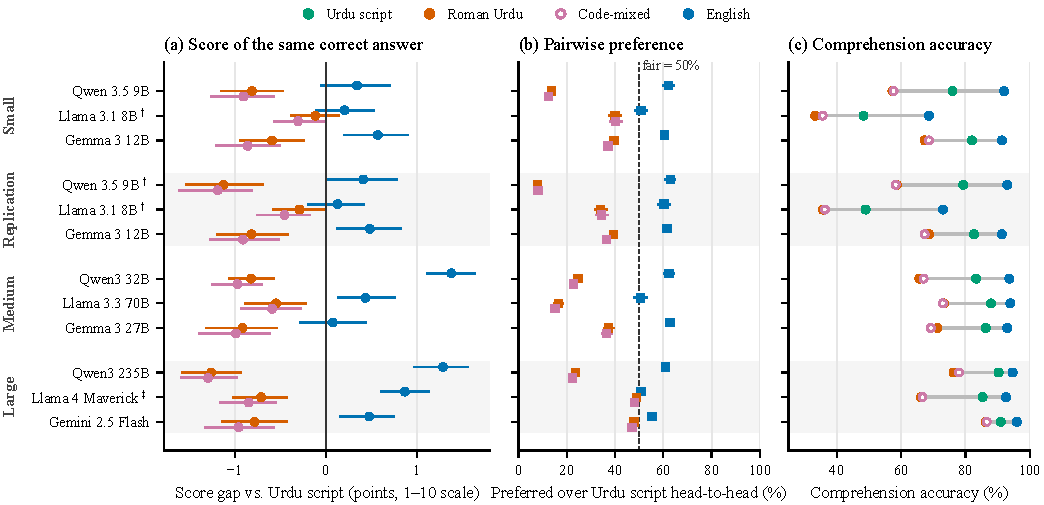
\includegraphics[width=\textwidth]{figures/results_overview.pdf}
\caption{Results for every judge, with 95\% confidence intervals. (a) Mark for the same correct answer compared with
Urdu script. (b) How often each version is chosen over the Urdu-script version (50\% is fair). (c) Reading accuracy.
$^\dagger$Failed the first check. $^\ddagger$Comparison result from the extra run.}
\label{fig:overview}
\end{figure*}

\subsection{Gap in marks (RQ1)}
Table~\ref{tab:main} and Fig.~\ref{fig:overview}a show the main result. Every judge that passed the first check gave the
same correct answer fewer marks in Roman Urdu ($-0.55$ to $-1.26$) and in mixed text ($-0.59$ to $-1.30$) than in Urdu
script. For all of them the confidence interval does not include zero. English answers got more marks, up to $+1.38$.
The average of the judges in each round shows the same gap ($-0.51$ to $-0.92$), and Round~2 gave the same pattern as
Round~1 with slightly bigger gaps.

In the comparison test (Fig.~\ref{fig:overview}b), most judges chose the Urdu-script answer. The Qwen models chose Roman
Urdu in only 8--25\% of cases, and Llama~3.3~70B in 17\%. Gemini~2.5~Flash and Maverick (extra run) said TIE about 95\% of
the time. When they did choose, though, they mostly chose Urdu script: Gemini 54 times out of 55, and Maverick 43 times
out of 61.

Wrong answers also passed more often in Roman Urdu. Llama~3.3~70B gave 7 or more to 57\% of wrong Roman Urdu answers but
to only 34\% of wrong Urdu-script answers, and its AUC fell from 0.81 to 0.66.

\subsection{Understanding (RQ2)}
Most judges are about 15 points less accurate when they answer questions in Roman Urdu (Fig.~\ref{fig:overview}c). To see
if this causes the gap, we kept only the questions that a judge answered correctly in both scripts. The gap was still
there, from $-0.57$ (Gemini~2.5~Flash) to $-1.35$ (Qwen3-235B), and no confidence interval included zero.

\begin{figure}[t]
\centering
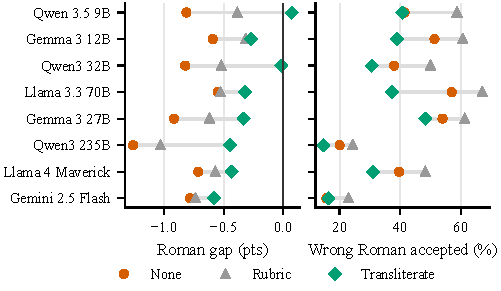
\includegraphics[width=\columnwidth]{figures/mitigations.pdf}
\caption{Fixes for the judges that passed the first check. Left: gap in marks for Roman Urdu. Right: share of wrong
Roman Urdu answers that got 7 or more.}
\label{fig:mitig}
\end{figure}

\subsection{Model size and fixes (RQ3)}
Bigger judges were better at telling correct and wrong answers apart (AUC in Urdu script of 0.57--0.74 for small models
and 0.81--0.87 for large ones), but their gap for Roman Urdu was not smaller. The biggest gap in the study came from the
biggest model, Qwen3-235B. Of the fixes (Fig.~\ref{fig:mitig}), changing the text into Urdu script first worked best. In
Rounds~1 and~3 the gap was no longer significant for four of the five small and medium judges that passed the first
check, and fewer wrong answers passed. The large judges still had a gap of $-0.43$ to $-0.58$. The line about ignoring spelling mostly made
judges give higher marks to everything. The gap became a little smaller, but every judge also passed more wrong answers
(Qwen~3.5~9B went from 41\% to 59\%).

% =====================================================================
\section{Remaining Work}
\label{sec:remaining}
For the final paper we plan to:
\begin{enumerate}
\item ask people who know both scripts to check 100 of the generated options and to mark a set of answers, so we can
compare the judges with human marks \cite{hada2024large};
\item test if asking judges to reason first makes the gap smaller;
\item mark several common spellings of each Roman Urdu answer \cite{khan2022clustering};
\item check if answers that look less familiar to a model get bigger gaps \cite{wataoka2024self};
\item write the reading passages in our own Roman Urdu too, and add free-text student answers.
\end{enumerate}

% =====================================================================
\section{Conclusion}
In all four rounds, LLM judges gave fewer marks to correct answers written in Roman Urdu or mixed text than to the same
answers in Urdu script, and they let more wrong Roman Urdu answers pass. For now, anyone who uses an LLM judge for Urdu should report results for each script separately, and should
change Roman Urdu into Urdu script or have a person check the marks.

\section*{Use of AI Tools}
We used AI tools in this project. Claude Opus~5.5 (Anthropic) wrote the Roman Urdu and mixed versions of the answer
options (Section~\ref{sec:data}). Claude, through the Claude Code tool, wrote most of the code for the testing website and
the analysis scripts under our direction, ran the experiments, made the figures and helped us draft and edit this paper.
The research question, the literature review and the plan of the study are our own. We checked the results and the text,
and we take full responsibility for this paper.

\bibliographystyle{IEEEtran}
\bibliography{references}

\end{document}
